\chapter{Case study: Central heating and pollution level}
\label{chap:case-staudyAC}

\section{Description case study}
Nowadays air pollution is a very common problem of cities of all the world.
Two of the main strategies used to reduce the emission of polluting gas are traffic bans in strategic city's areas and maximum temperature allowed in public and private building heating control.

In this context we want to realize a monitoring system for the air quality based on the CAQI index~\cite{CAQI}, which is able to apply strategies to maintain under control the air pollution level.
The sensor network is composed of a set of fixed sensors scattered around the city, and mobile sensors placed on public transports (like bus or public bicycles).
The idea is to displace strategically the fixed sensors to achieve a good city coverage, using mobile sensors for its refinement and reduce reading errors of the fixed ones.

In a first step to reduce air pollution it has chosen to control the maximum temperature allowed for the heating of buildings.
The idea is to allow the system to manage the building heating systems control devices (from now on building devices). So the system can set the maximum reachable temperature based on the area pollution level.

All the sensors have to be displaced in a LoRaWAN network to communicate their sensed data to reduce their cost and the cost for their maintenance. 
Building devices have not any particular requirements, they have not problems of energy consumption because they can be connected to the power line of the building.
The same policy can be adopted for the Internet connection, this allow to avoid to use LoRa technology reducing the number of LoRa devices in the network and increasing their communication capability.

\section{Design of the system}

Aggregate computing is a good approach for this system for several reasons, it is a heterogeneous system composed for at least two type of device (sensor and building device) with different capabilities like connectivity, computational resources, and how they can interact with the environment. 
Furthermore it is composed from an high number of devices (one device building for each house of the city, a set of fixed sensors and one set of mobile ones) so scalability can be a problem, but with aggregate computing is possible to solve it scaling horizontally and moving the computational node in different network devices without the need to change the aggregate program.

\autoref{fig:caseStudyAC} shows a high level architecture of the system
\begin{figure}[h]
    \centering
    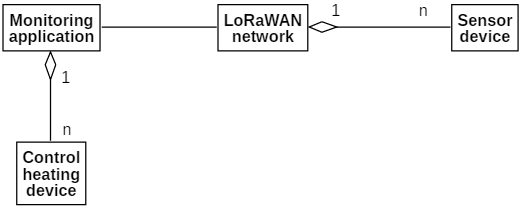
\includegraphics{figures/ACapp.png}
    \caption{High level architecture of the system}
    \label{fig:caseStudyAC}
\end{figure}

\subsection*{Entities model}

\subsection*{Interaction between Protelis nodes}
% network manager - policy vicinato - vicinato aggiornato automamente

\section{Protelis program}
\lstinputlisting[
	float,
	language=Protelis,
	caption={Protelis program for monitoring application},
	label={lst:program},
]{listings/homeHeating_timer.pt}

\section{Simulation in DingNet}